\documentclass{article}

\usepackage{enumitem}
\usepackage{tikz}
\usetikzlibrary{automata, positioning}


\newlist{qanda}{enumerate}{1}
\setlist[qanda,1]{label=\textbf{Q\arabic*:}, 
                  left=0pt, 
                  itemsep=1em, 
                  align=left, 
                  wide=0pt}

\newcommand{\answer}[1]{\\\textbf{A:} #1}

\title{Theory of Computation}
\author{Mohammed Fahad}

\begin{document}

\maketitle

\section{Why TOC?}

\begin{itemize}
    \item It helps us to understand the limits of what computer can do and how to model computation using mathematics
\end{itemize}

\begin{qanda}
    \item What is the motivation for studying theory behind computation? OR Needs of TOC?
    \answer{
        \begin{itemize}
            \item Understanding the capability of a computer
            \item To find steps to solve a problem
            \item Increase efficiency while doing a task
        \end{itemize}
    }

    \item List the problems that cannot be solved by a computer.
    \answer{
        \begin{enumerate}
            \item Ethical problems. Eg: Self-driving car deciding to save the driver/passenger or the pedestrian
            \item Generating truly original art of emotion
        \end{enumerate}
    }

\end{qanda}

\section*{Automaton (pl.: Automata)}

A simplified mathematical model of a machine (digital computer). It 
\begin{itemize}
    \item Accepts input
    \item Produces output
    \item Nay have some temporary storage
    \item can make descisions in transforming the input into the output
\end{itemize}

\begin{qanda}
    \item Why study computability and theory?
    \answer{
        \begin{itemize}
            \item It helps to answer: "Can this be solved by a computer?"
            \item Understand the principles behind algorithms and programs
            \item Explore the boundary between what is possible and impossible in computing
        \end{itemize}
    }
\end{qanda}

\subsection{Need for mathematical modelling}
\begin{itemize}
    \item Computers work on rules \& logic
    \item We can represent computers using abstract models
    \item These models helps us study complex behaviour in a simplified way
\end{itemize}

\section{Introduction to finite automata}

\begin{enumerate}
    \item ON/OFF Switch:
        \begin{center}
        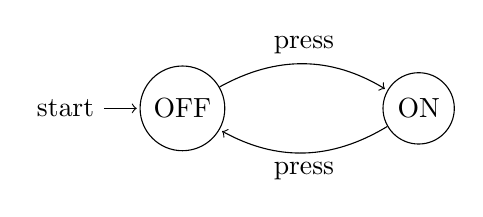
\begin{tikzpicture}[shorten >=1pt, node distance=3cm, on grid, auto]

        \node[state, initial] (OFF) {OFF};
        \node[state, right=of OFF] (ON) {ON};

        \path[->]
            (OFF) edge[bend left] node {press} (ON)
            (ON) edge[bend left] node {press} (OFF);

        \end{tikzpicture}
        \end{center}
    \item Coffee vending machine (Inputs: Rs. 5 \& Rs. 10 | Rs. 15 for one coffee):
        \begin{center}
        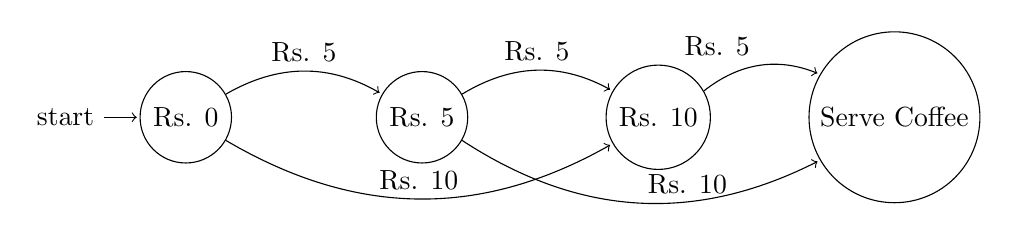
\begin{tikzpicture}[shorten >=1pt, node distance=3cm, on grid, auto]

        \node[state, initial] (NONE) {Rs. 0};
        \node[state, right=of NONE] (FIVE) {Rs. 5};
        \node[state, right=of FIVE] (TEN) {Rs. 10};
        \node[state, right=of TEN] (SERVE) {Serve Coffee};

        \path[->]
            (NONE) edge[bend left] node {Rs. 5} (FIVE)
            (FIVE) edge[bend left] node {Rs. 5} (TEN)
            (TEN) edge[bend left] node {Rs. 5} (SERVE)
            (NONE) edge[bend right] node {Rs. 10} (TEN)
            (FIVE) edge[bend right] node {Rs. 10} (SERVE);
        \end{tikzpicture}
        \end{center}


\end{enumerate}

\section{Formal Language}
A formal language is an abstraction of the general characteristics of programming langauges.

A formal language consists of set of symbols and some rules of formation by which these symbols can be combined into entities called sentences.

\end{document}
